\documentclass[../thesis.tex]{subfiles}
 
\begin{document}
\vspace{-1\baselineskip}

Reconstruction software reconstructs basic objects from signals collected from the event: interaction vertices, tracks, topological clusters of energy deposits\\
These quantities then used to reconstruct physics objects i.e. particles (electron, muon), jets, MET

\section{Primary reconstruction}
\label{sec:primaryreco}

\subsection{Topological clusters}
\label{sec:topocluster}
\citep{reco:topocluster}\citep{reco:topocluster_2}\\
Topological cluster (topo-cluster): Clusters of topologically connected cell signals in the calorimeter at the EM scale. This scale does not consider loss of signal from hadrons. Singular hits without hits from neighboring cells are considered noise.\\
Done in an effort to extract signal while minimizing electronic effects and physical fluctuations. 
Used to reconstruct hadronic objects and particles decaying hadronically i.e. $\tau$ leptons\\
Signal hits with significance above a cell signal significance level $\varsigma_\mathrm{cell}^\mathrm{EM}$ are seeded in as part of a proto-cluster. Neighboring cells satisfying a cluster growth threshold are collected into the cluster.\\
Two clusters are merged if a cell is matched to both\\
If a cluster has two or more local signal maxima satisfying $E_\mathrm{cell}^\mathrm{EM}>500$ MeV, the cluster is split accordingly.\\
The process continues iteratively until all cells with significant signal efficiency have been matched to a cluster.\\
\begin{figure}[!htbp]
\begin{center}
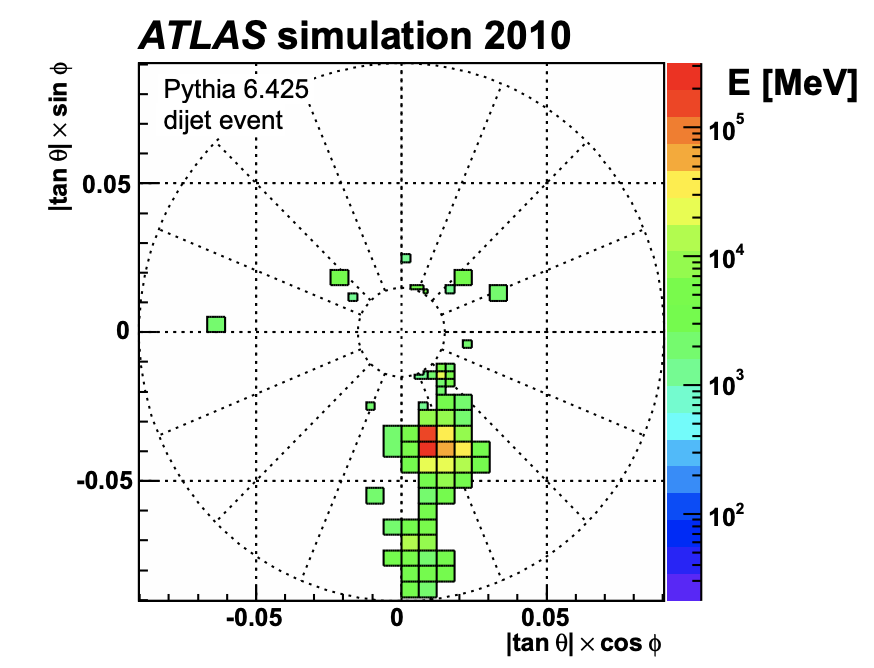
\includegraphics[width=\linewidth]{fig/reco_topo1.png}
\caption{\label{fig:reco:topo1}}
\end{center}
\end{figure}

\subsection{Tracks}
\citep{reco:track}\\
Charged particles deposit energy in different layers of the inner detector and muon spectrometer\\
ID reco software: inside-out and outside-in algorithms\\
\begin{itemize}

\item Inside-out: \citep{reco:io}\\
Starts with seeded hits in the silicon detector in pixel \& SCT\\
Loosely matched to an EM cluster to form a track candidate\\
Hits are added to form a track candidate using a pattern recognition algorithm based on a Kalman filter formalism \citep{reco:kalman}\\
Track candidates are then fitted with a $\chi^2$ filter \citep{reco:track_chi2} and loosely matched to a fixed-sized EM cluster. Successfully matched track candidates are re-fitted with a Gaussian-sum filter (GSF) \citep{reco:track_gsf}\\
This is followed by a track scoring strategy to resolve fake tracks \& hit ambiguity between different tracks \citep{reco:track_ambiguity}\\
Extend to TRT to form final tracks, filtered by threshold $\pT > 400$ MeV.\\
\item Outside-in: \citep{reco:oi}\\
Reverse, starts with segments in TRT extending inward to silicon hits in pixel \& SCT\\
Targeting secondary tracks (decays/interactions of primary particles) or long-lived particles
\end{itemize}

\subsection{Vertices}
Vertices: interaction or decay point\\
Primary vertex: pp interaction point\\
%Secondary vertex: secondary interaction or decay long-lived particle\\
Important for reconstruction of the hard scattering pp interaction, resulting trajectories and kinematic information of the event\\
\begin{itemize}
\item Vertex finding:\\
Uses the z-position of a track as input\\
Vertices require to have at least 2 tracks\\
Iterative $\chi^2$ algorithm evaluate track-vertex compatibility, using the track as new seed for another vertex if large discrepancy
\item Vertex fitting:\\
Adaptive multi-vertex fitter (AVF) algorithm assigns weights that depend on the track-vertex compatibility to each track to measure the probability of the track being an outlier vs inlier.\\
Vertex is then estimated by iteratively minimizing an objective function of these weights
\end{itemize}


\section{Jets}
- Quarks, gluons \& other non-color-neutral hadrons cannot be observed individually due to QCD color confinement\\
- A non-color-neutral hadron will almost immediately undergo hadronization producing a cone of color-neutral hadrons also known as a jet\\
- Jet signals can be used to reconstruct and consequently indirectly observe the original quarks/gluons the jets originated from\\
- Jet reconstruction:
\begin{itemize}
\item PFlow: energy deposited in the calorimeter systems by charged particles is removed and replaced by particle objects created with the remaining energy in the calorimeter and tracks matched to the topo-clusters. (include PFlow graphics)
\item anti-$k_t$ algorithms: sequential recombination jet algorithms
\item pile-up jets: multiple interactions associated with one bunch crossing in addition to the hard scattering of interest and reconstructed as jets in the final states. Reconstructed pile-up jets can result from   Pile-up jets are usually from soft interactions and can be distinguished with JVT algorithm using tracking information from the ID.
\item JES/JER calibration: Jet reconstruction at EM scale does not accurately account for energy from QCD interactions and needs to be calibrated to jets reconstructed at particle level. This is done via a MC-based JES calibration sequence and additional JER calibration to match jet resolution in simulation to data using dijet events.
%\item reco setting: PFlow and anti-$k_t$ algorithms with radius parameter $R=0.4$, JVT applied to reconstructed jets with $\pT < 60$ GeV and $|\eta|<2.4$.
\end{itemize}
\subsection{Flavor tagging}
\label{sec:ftag}
- Classification of hadronic jets is an important task for many LHC analyses especially ones studying final states (Higgs decay/4top)\\
- Flavor tagging is namely interested in identifying jets containing $b$-hadrons, $c$-hadrons, $uds$-hadrons (light-jets), and hadronic decays from $\tau$.\\
- Of these, identifying $b$-jets is of particular interest due to their characteristically long lifetime ($\approx 1.5$ ps) from decay suppression by CKM factor, with a displaced secondary decay vertex and usually a tertiary vertex from $c$-hadron decays.




\subsubsection*{Efficiency calibration}
- \citep{ftag:calib}\\
- Performance of $b$-taggers are studied on MC simulated samples. However, the $b$-tagging efficiency predicted by simulation $\varepsilon_b^\mathrm{sim}$ is usually not the same as the efficiency measured in data $\varepsilon_b^\mathrm{data}$.\\
- The correction for the rate of events after applying a $b$-tagging requirement is calibrated and applied jet by jet in the form of data-to-simulation scale factors $\mathrm{SF}=\varepsilon_b^\mathrm{data}/\varepsilon_b^\mathrm{sim}$.\\
- Usage of $b$-tagger in this analysis is done via five operating points (OPs), corresponding to 60\%, 70\%, 77\%, 85\% and 90\% $b$-jet tagging efficiency $\varepsilon_b$ in simulated \ttbar events in order from loosest to tightest discriminant cut points.
- OPs are defined by selection on the tagger output to provide a pre-defined level of $\varepsilon_b$, and act as a variable trade-off between $b$-tagging efficiency and $c$-/light-jet rejection i.e. $b$-jet purity \\
- A jet is considered $b$-tagged if it passes the efficiency criteria for a given OP. A pseudo-continuous $b$-tagging (PCBT) score is defined to summarize the OP criteria a jet passes into a variable. The PCBT score can take integer values between 1 and 6, where a score of 6 means a jet passes all four OP thresholds (passing 65\% OP), a score of 2 for jets that pass only the 90\% OP, and a score of 1 for jets that don't pass any OP. Additionally, PCBT defines a value of -1 for any jet that does not satisfy $b$-tagging criteria.\\
- (insert TPR/FPR discriminant trade-off figure)\\
\\
\\
\\
- ttbar calibration \citep{ftag:ttbar}\\
- ptrel and high pT calibration \citep{ftag:multijet}\citep{ftag:highpt}\citep{ftag:ptrel}\\
- impact parameter \verb|->| signed transverse impact parameter significance\\
- calibration results




\subsubsection*{GN2 $b$-tagging algorithm}
\label{sec:btag}
\begin{figure}[!htbp]
\begin{center}
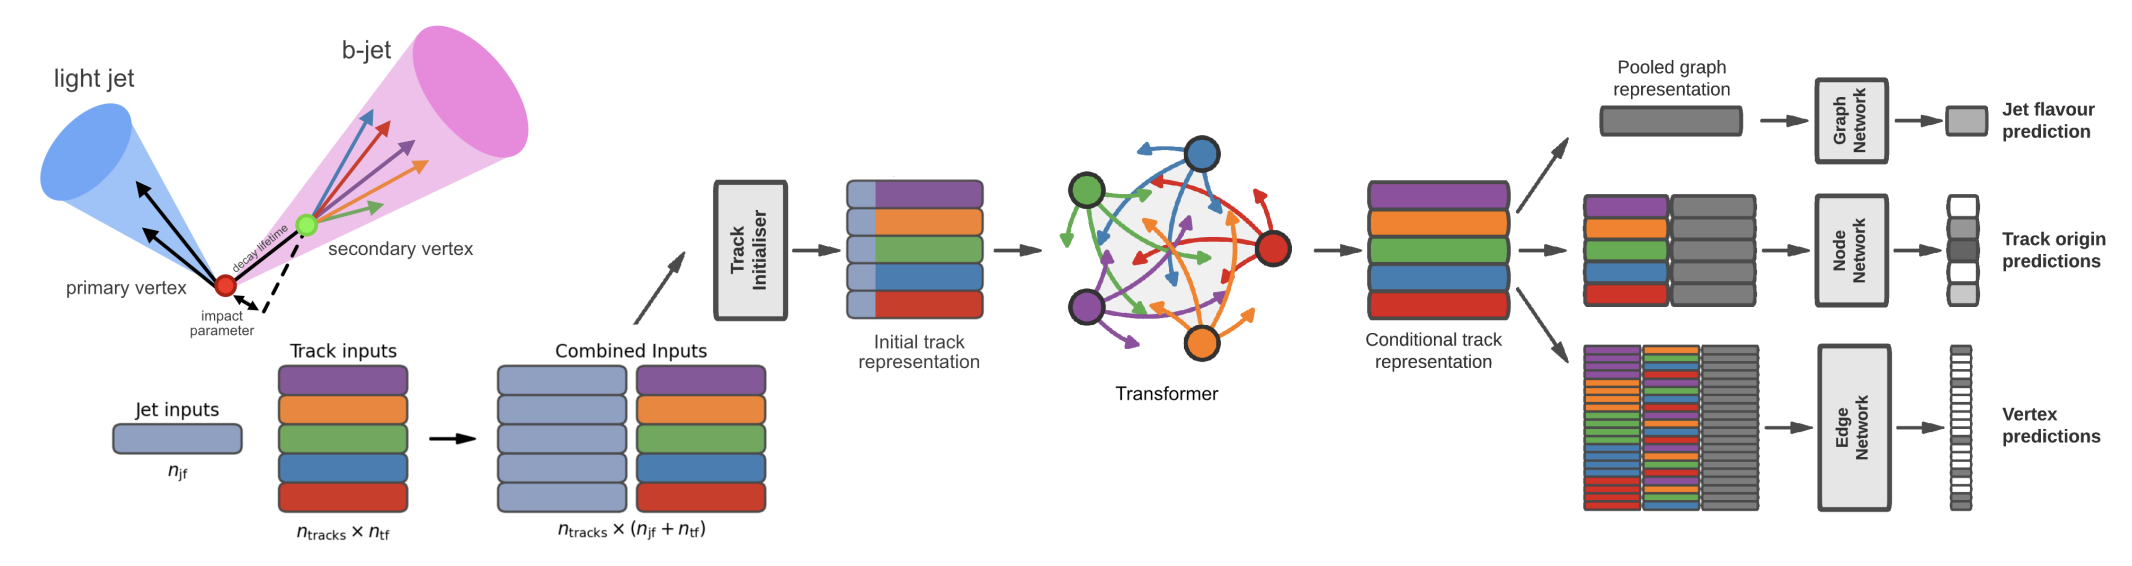
\includegraphics[width=\linewidth]{fig/ftag_gn2.png}
\caption{\label{fig:ftag:gn2} \citep{ftag:gn1}\citep{ftag:gn1.1}\citep{ftag:gn2}}
\end{center}
\end{figure}

- GN2 transformer-based $b$-tagging algorithm, utilized for analysis of Run 2 and Run 3 data\\
- GN2 gives a factor of 1.5-4 improvement in experimental applications compared to the previous convolutional neural network-based standard $b$-tagging algorithm, DL1d, without dependence on the choice of MC event generator.\\
- Attention-based architecture, modified to incorporate domain knowledge and additional auxiliary physics objectives: grouping tracks originating from common vertices and prediction of the underlying process for each track\\
- MC simulated SM \ttbar and BSM $Z'$ events from $pp$ collisions were used as training and evaluation samples. In order to minimize bias, both $b$- and light-jet samples are re-sampled to match $c$-jet distributions. \\
- GN2 concatenates 2 jet and 19 track reconstruction variables of up to 40 tracks to form the input feature vector, normalized to zero mean and unit variance.\\
- The output consists of a jet classification layer of size 4 consisting of $p_b$, $p_c$, $p_u$ and $p_\tau$ for the probability of each jet being a $b$-, $c$-, light- or $\tau$-jet respectively; a track-pairing output layer of size 2, and a track origin classification layer of 7 output categories. 

\section{Leptons}
- Lepton reconstruction is concerned mainly with electron and muon construction, since tau decays quickly and can either be reconstructed using jets or light leptons. From here on out lepton will be used mostly to refer to electrons and muons\\
- Leptons can be classified into two categories: prompt leptons resulting from heavy particle decays, or non-prompt leptons resulting from detector or reconstruction effects, or from $b$- or $c$- hadron decays\\
- Reconstruction of leptons is therefore important to study the underlying physics and suppressing background
\subsection{Electrons}
- \citep{reco:electron_id}\citep{reco:electron_meas}\\
- Electrons lose energy interacting with the detector materials via bremsstrahlung. The bremsstrahlung photon can then produce an electron-positron pair which can itself leaves signals in the detector, creating a collimated object that can leave multiple tracks in the ID or EM showers in the calorimeter, all considered part of the same EM topo-cluster.\\
- Electron signal signature has three characteristic components: localized energy deposits in the calorimeter, multiple tracks in the ID and compatibility between the above tracks and energy clusters in the $\eta \times \phi$ plane. Electron reconstruction in ATLAS follows these steps accordingly
\begin{figure}[!htbp]
\begin{center}
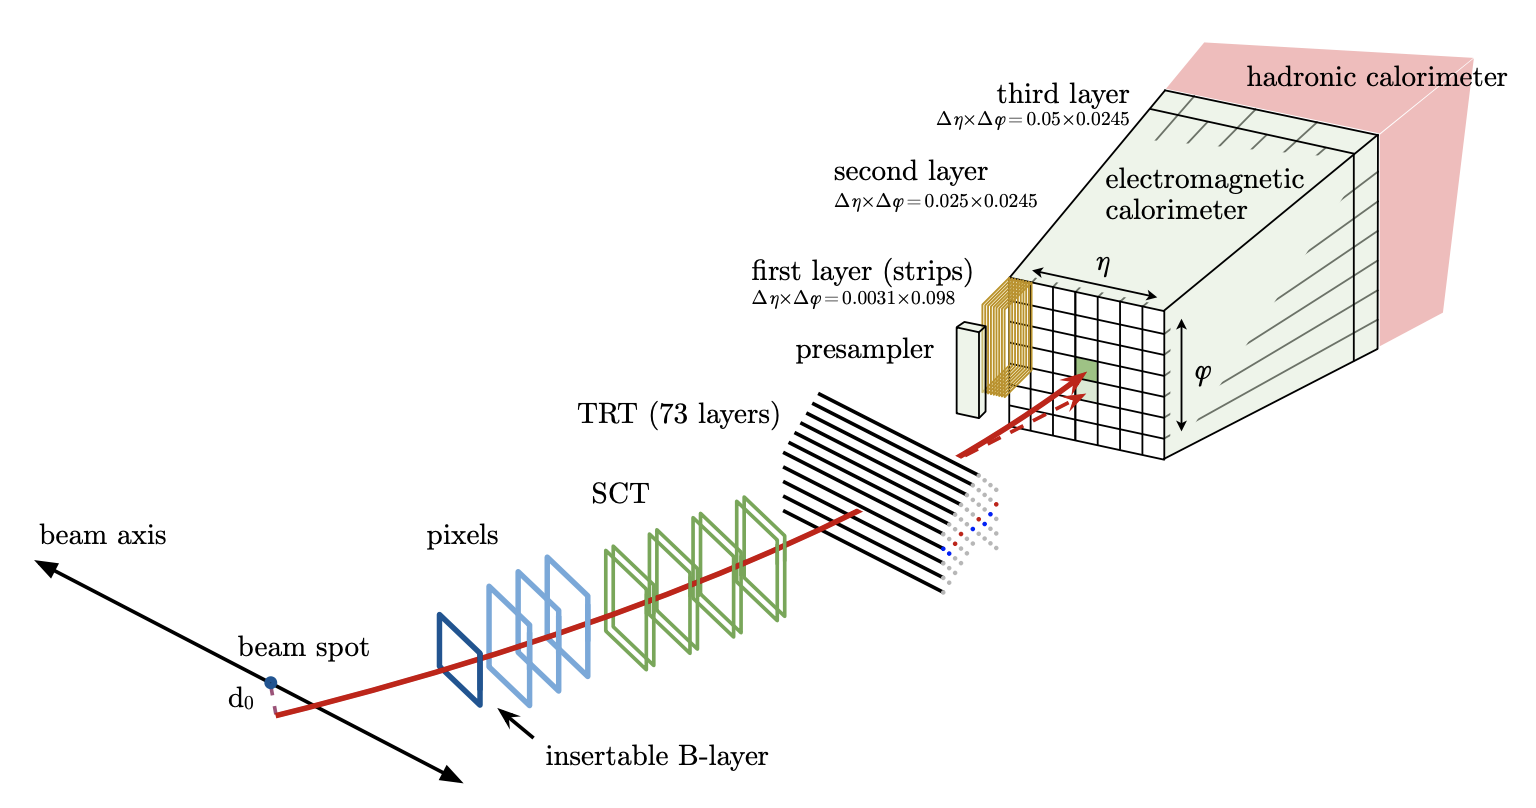
\includegraphics[width=\linewidth]{fig/reco_electron.png}
\caption{\label{fig:reco:electron}\citep{reco:electron_id}}
\end{center}
\end{figure}
- Seed-cluster reconstruction and track reconstruction are performed sequentially in accordance with the iterative clustering algorithm and track reconstruction method respectively, described in \autoref{sec:primaryreco}\\
- The seed-cluster and track candidate associated with a conversion vertex are then matched to form an electron candidate.\\
- A reconstructed cluster is expanded from the seed-cluster in either $\phi$ or $\eta$ in the barrel or endcap region respectively\\
- The cluster energy is then calibrated to compute the original electron energy.

\subsubsection*{Electron identification}
- Additional likelihood-based identification selections using ID and EM calorimeter information are implemented to further improve the purity of the reconstructed electrons and photons. These selections also help suppress background from hadronic jet deposits, photon conversions or electrons from heavy-flavor decays.\\
- Three operating points are defined for physics analyses: Loose, Medium and Tight, optimized for 9 bins in $|\eta|$ and 12 bins in \ET with each corresponding to a fixed efficiency requirement for each bin. The target efficiencies for Loose, Medium and Tight start at 93\%, 88\% and 80\% respectively for typical EW processes and increases with \ET \\ Similar to $b$-tagging OPs, the electron OPs represent a trade-off in signal efficiency and background rejection. The electron efficiency are estimated using tag-and-probe method \citep{reco:electron_id} on samples of $J/\Psi \rightarrow ee$ and $Z \rightarrow ee$.
%The analysis in this thesis uses Tight electron identification requirement.
\begin{figure}[!htbp]
\centering
\subfloat[Figure A]{
\label{fig:a}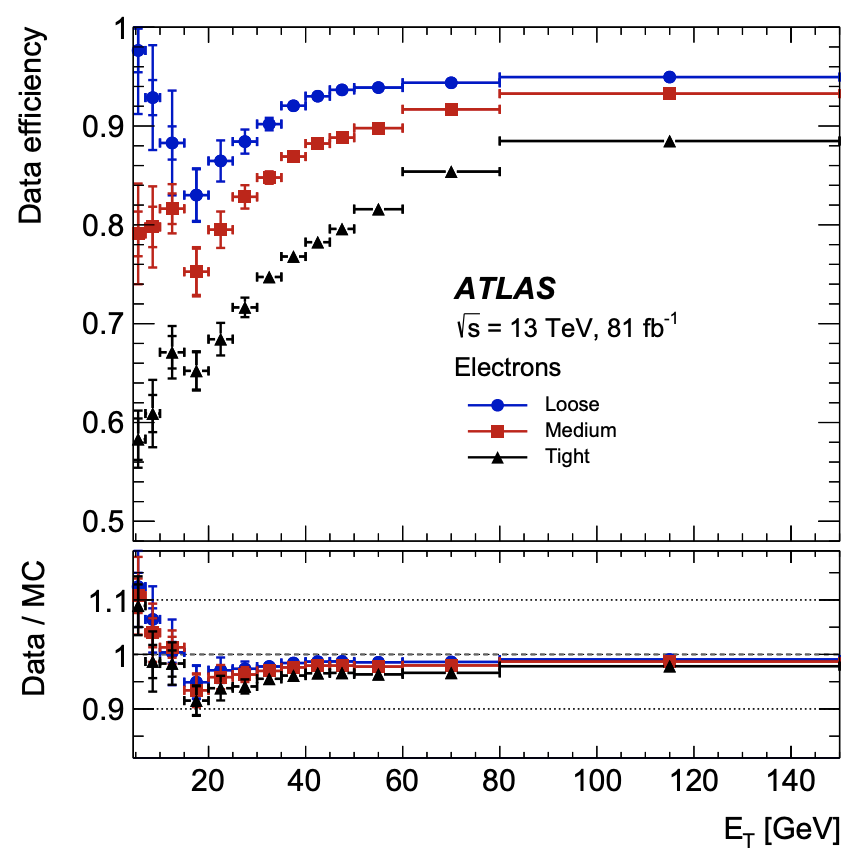
\includegraphics[width=0.5\linewidth]{fig/reco_electron_eff_ET.png}}
\subfloat[Figure B]{
\label{fig:b}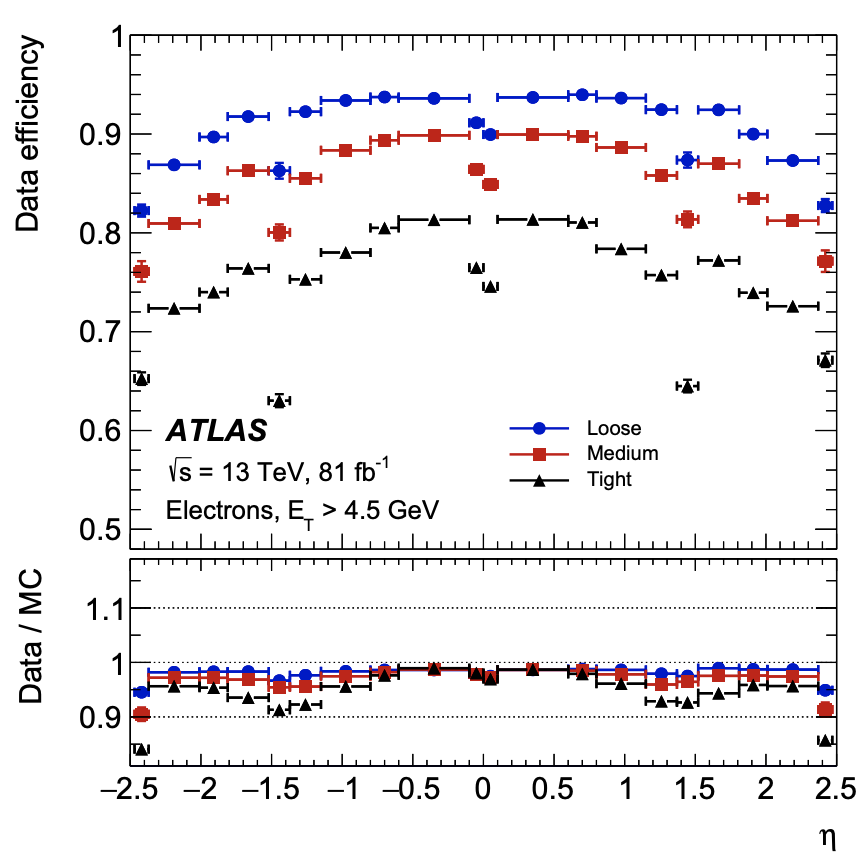
\includegraphics[width=0.5\linewidth]{fig/reco_electron_eff_eta.png}}
\caption{\label{fig:reco:electron_eff}\citep{reco:electron_meas}}
\end{figure}

\subsubsection*{Electron isolation}
\label{sec:eiso}
- A characteristic distinction between prompt electrons and electrons from background processes is the relative lack of activity in both the ID and calorimeter within an area of $\Delta \eta \times \Delta \phi$ surrounding the reconstruction candidate\\
- Electron isolation variables are needed to quantify the amount of activity around the electron candidate.\\
- Calorimeter-based isolation variables $E_\mathrm{T}^{\mathrm{cone}XX}$ is calculated by first summing the energy of topological clusters with barycenters falling within a cone of radius $\Delta R = \sqrt{(\Delta \eta)^2+(\Delta \phi)^2}=XX/100$ around the direction of the electron candidate.\\
- The final isolation variable is then obtained by subtracting energy at the core of the cone belonging to the candidate electron from the sum, then applying corrections for energy leakage outside of the core and pile-up effects.\\
- Similar to calorimeter-based variables, track-based isolation variables $p_\mathrm{T}^{\mathrm{varcone}XX}$ are calculated by summing all track \pT within a cone of variable radius $\Delta R$ around the electron candidate, minus the candidate's contribution. The cone radius is variable as a function of \pT
$$\Delta R = \min \left(\frac{10}{\pT \mathrm{ [GeV]}}, \Delta R_{\max} \right)$$
with $\Delta R_{\max}$ being the maximum cone size, to account for the closer proximity of decay products to the electron in high-momentum heavy particle decays.\\
- Four isolation operating points are implemented to satisfy specific needs by physics analyses: Loose, Tight, HighPtCaloOnly and Gradient. The first three OPs are fixed in isolation variables, while the Gradient OP fixes the isolation efficiency to a \pT dependent function defined as $ \varepsilon = 0.1143 \times \pT + 92.14\% $ with \pT in GeV, using $\Delta R=0.2$ for calorimeter isolation and $\Delta R_{\max}=0.2$ for track isolation.
%For this thesis, electrons isolation using Tight requirements.

\begin{figure}[!htbp]
\centering
\subfloat[Figure A]{
\label{fig:a}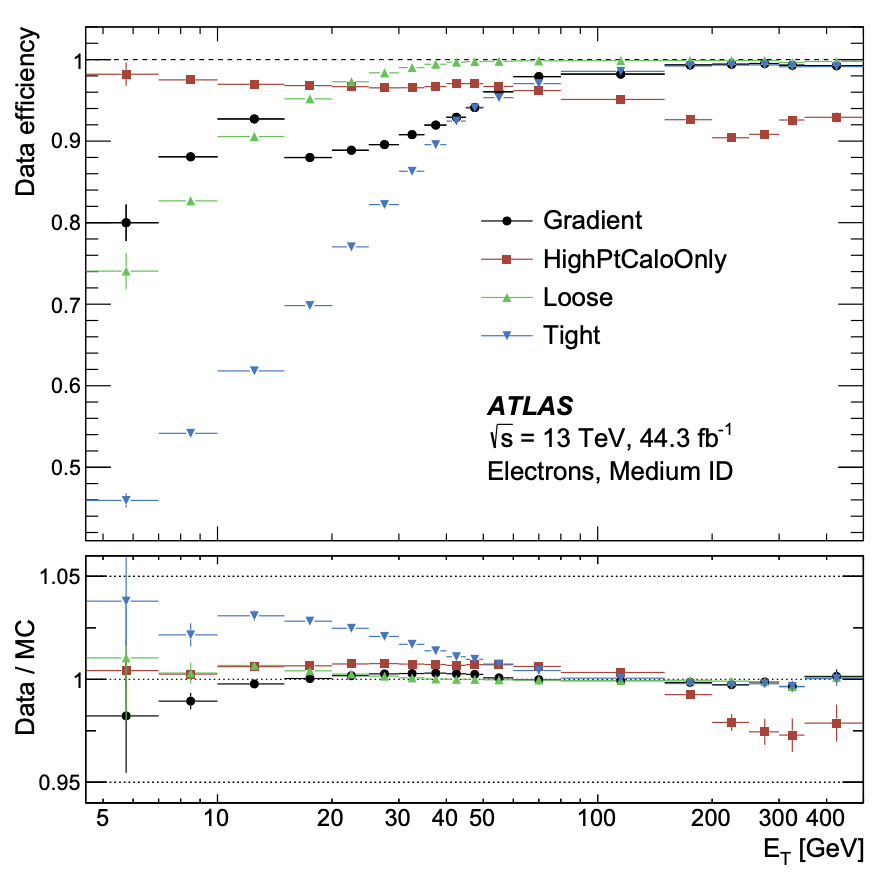
\includegraphics[width=0.5\linewidth]{fig/reco_electron_iso_ET.png}}
\subfloat[Figure B]{
\label{fig:b}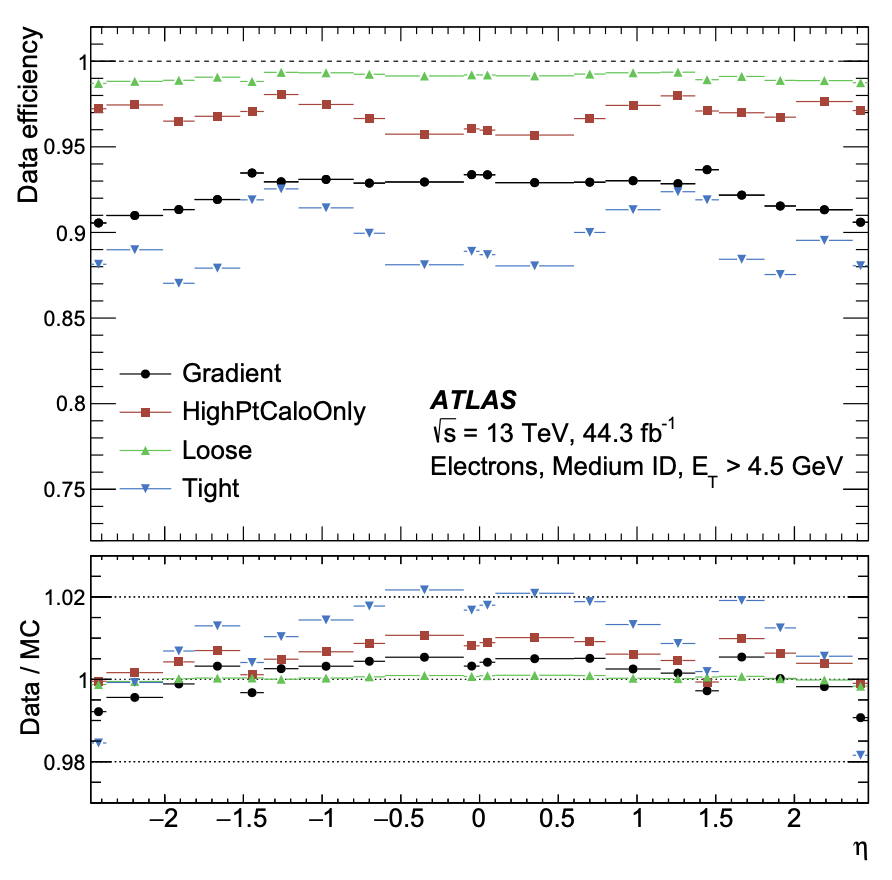
\includegraphics[width=0.5\linewidth]{fig/reco_electron_iso_eta.png}}
\caption{\label{fig:reco:electron_iso}\citep{reco:electron_meas}}
\end{figure}

\subsubsection*{Electron charge misidentification}
\citep{reco:electron_id}\citep{reco:qmisid_cnn}\\
Electron charge is determined by the curvature of the associated track. Misidentification of charge can then occur via either an incorrect curvature measurement, or an incorrectly matched track.\\
The former is more likely for electrons with high \pT due to the small curvature in track trajectories at such scale, while the latter usually results from bremsstrahlung pair-production, creating additional secondary tracks in the vicinity.\\
Charge misidentification is a crucial irreducible background for analyses with charge selection criteria, and suppression of this background is assisted via a boosted decision tree discriminant known as the Electron Charge ID Selector (ECIDS) \citep{reco:electron_id}. The addition of ECIDS removed 90\% of electrons with incorrect charge while selecting 98\% of electrons with correct charge from electrons in $Z\rightarrow ee$ events satisfying Medium/Tight identification and Tight isolation criteria.
\begin{figure}[!htbp]
\centering
\subfloat[Figure A]{
\label{fig:a}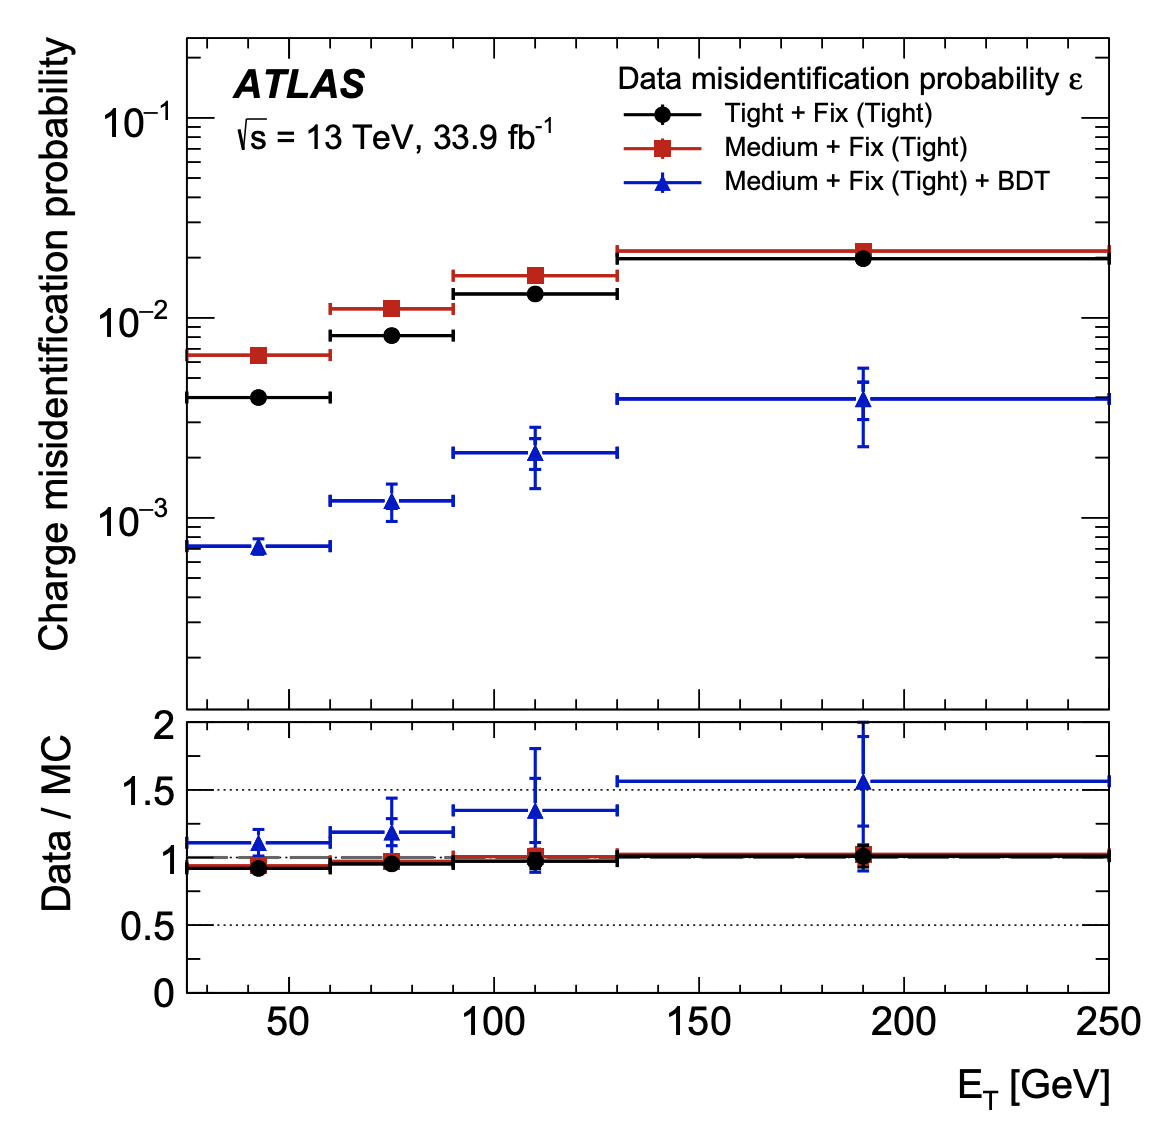
\includegraphics[width=0.5\linewidth]{fig/reco_qmisid_ET.png}}
\subfloat[Figure B]{
\label{fig:b}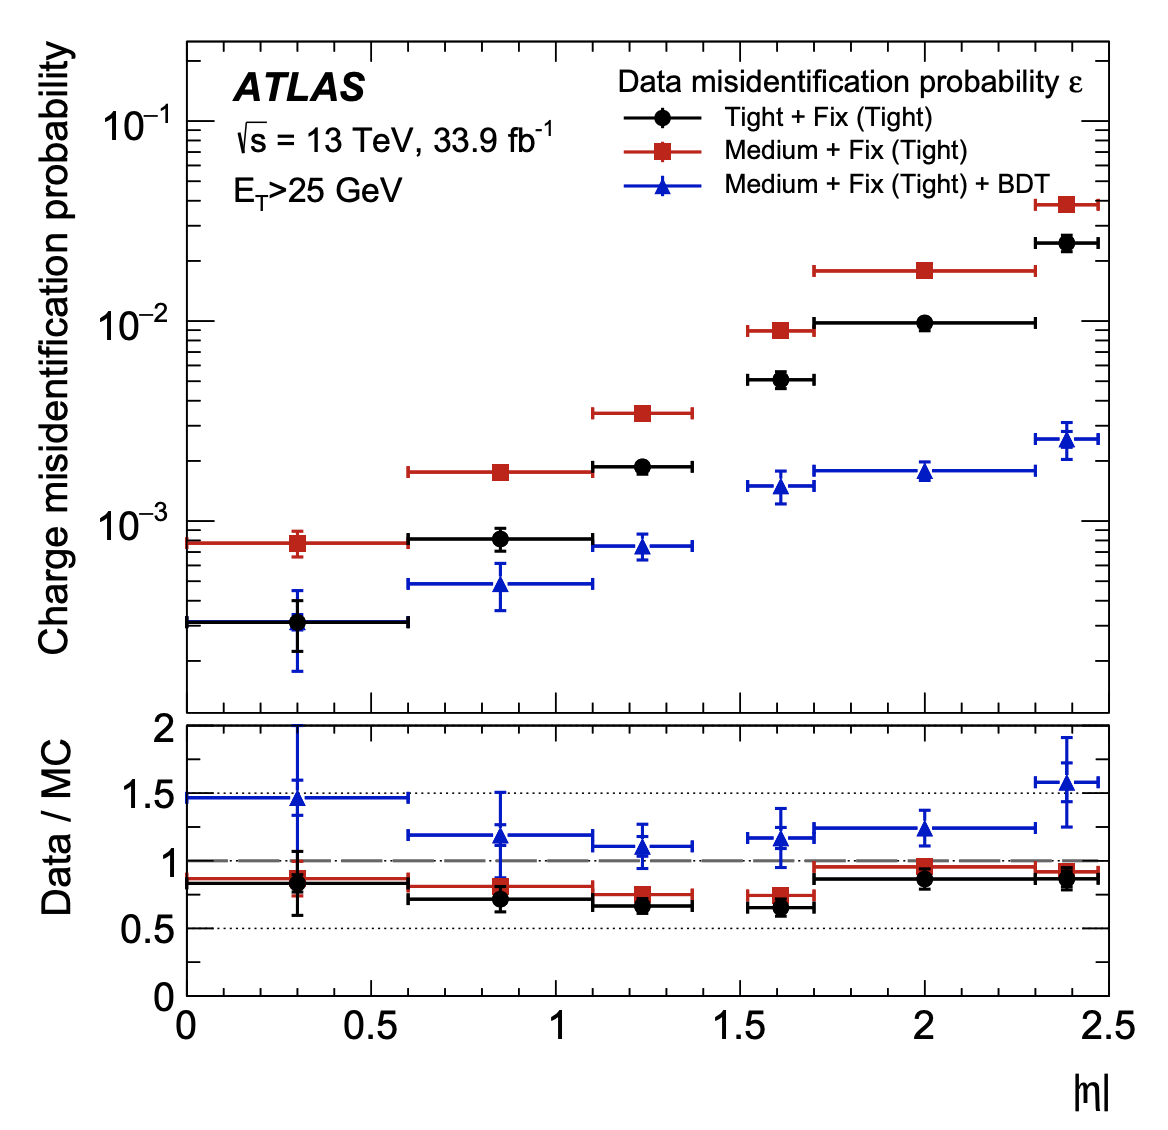
\includegraphics[width=0.5\linewidth]{fig/reco_qmisid_eta.png}}
\caption{\label{fig:reco:electron_iso}\citep{reco:electron_meas}}
\end{figure}


\subsection{Muons}
Signature: minimum-ionizing particle leaves tracks in the MS or characteristics energy deposits in the calorimeter\\
Muons can be reconstructed globally using information from the ID, MS and calorimeters.\\
Five reconstruction strategies, each corresponding to a muon type:
\begin{itemize}
\item Combined (CB): primary ATLAS muon reconstruction method. Muons first reconstructed using MS tracks then extrapolated to include ID tracks (outside-in strategy). A global combined fit is then performed on both MS and ID tracks
\item Inside-out combined (IO): Complementary to CB algorithm. Muon tracks are extrapolated from ID to MS, then fitted together with a combined track fit. Useful for muons without good MS information.
\item MS extrapolated (ME): ME muons are defined as muons with a MS track that cannot be matched to an ID track using CB method. ME muons allow extension of muon reconstruction acceptance to regions not covered by the ID ($2.5<|\eta|<2.7$)
\item Segment-tagged (ST): ST muons are ID tracks satisfying tight angular matching criteria to at least one reconstructed local segment in the MDT or CSC chambers when extrapolated to the MS. Used primarily when muons only crossed one layer of MS chambers.
\item Calorimeter-tagged (CT): CT muons are ID tracks that when extrapolated through the calorimeter, can be matched to energy deposits consistent with those of a minimum-ionizing particle. Extends acceptance range to regions in the MS with sparse instrumentation ($|\eta|<0.1$), with a higher \pT threshold of 5 GeV compared to 2 GeV threshold used by other muon reconstruction algorithms due to large background contamination at the low \pT range of $15 < \pT < 100$ GeV
\end{itemize}
\subsubsection*{Muon identification}
\citep{reco:muon_ID}\citep{reco:muon_ID2}\\
Reconstructed muons are further filtered by identification criteria to select for high-quality prompt muons for physics analyses. Requirements include number of hits in the MS/ID, track fit properties and compatibility between measurements of the two systems.\\
Three standard WPs (Loose, Medium, Tight) are defined to better match the needs of different physics analyses concerning prompt muon ID efficiency, \pT resolution and non-prompt muon rejection. Of the three, Medium WP is the default ID WP for ATLAS, by virtue of being optimized in efficiency and purity for a wide range of analyses while minimizing non-prompt rejection and systematic uncertainties.\\

\begin{figure}[!htbp]
\centering
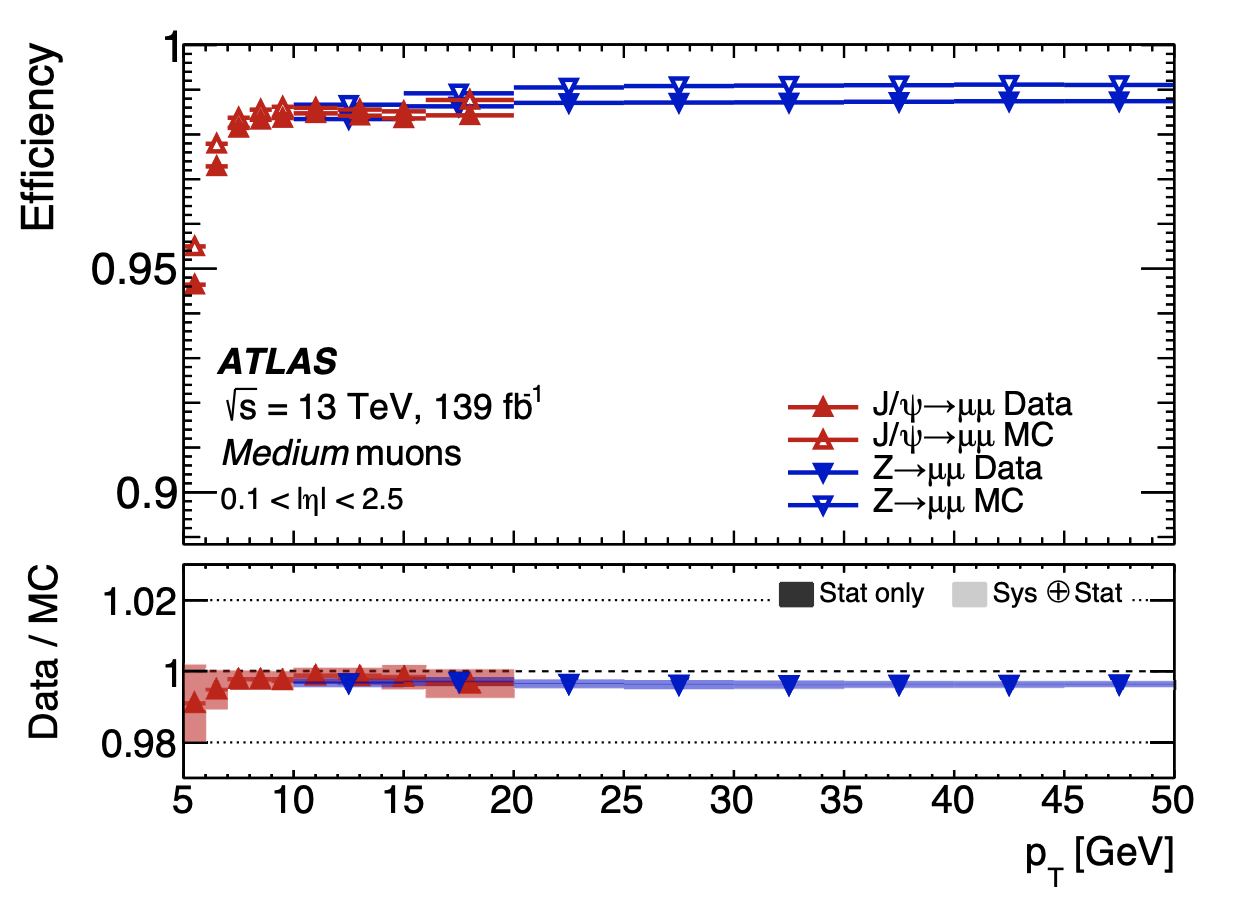
\includegraphics[width=0.9\linewidth]{fig/reco_muon_ID.png}
\caption{\label{fig:reco:muon_ID}\citep{reco:muon_ID}}
\end{figure}

\subsubsection*{Muon isolation}
Muons from heavy particle decays are often produced in an isolated manner compared to muons from semileptonic decays. Muon isolation is therefore an important tool for background rejection in physics analyses\\
Muon isolation strategies are similar to that of electron in \autoref{sec:eiso}, with track-based and calorimeter-based isolation variables.\\
Seven isolation WPs are defined to satisfy analyses' needs.

\section{Missing transverse momentum}
\label{sec:met}
\citep{reco:met}\\
Collisions at the LHC happen along the z-axis of the ATLAS coordination system between two particle beam of equal center-of-mass energy. By conservation of momentum, the sum of transverse momenta of outgoing particles should be zero. A discrepancy between measured momentum and zero would then suggest the presence of undetectable particles, which would consist of either SM neutrinos or some unknown BSM particles. This makes missing transverse momentum ($E_\mathrm{T}^\mathrm{miss}$) an important observable to reconstruct.\\
Reconstructing $E_\mathrm{T}^\mathrm{miss}$ utilizes information from fully reconstructed leptons, photons, jets and other matched track-vertex objects not associated with a prompt object (soft signals), defined with respect to the $x (y)$-axis as
\begin{equation}
E^\mathrm{miss}_{x (y)} = -\mathlarger{\sum}_{i \in \{\text{hard objects}\}} p_{x (y),i} -\mathlarger{\sum}_{j \in \{\text{soft signals}\}} p_{x (y),j},
\end{equation}
where $p_{x(y)}$ is the $x(y)$-component of \pT for each particle. The following observables can then be defined:
\begin{align}
& \mathbf{E}_\mathrm{T}^\mathrm{miss}=(E^\mathrm{miss}_{x},E^\mathrm{miss}_{y}),\\
& E_\mathrm{T}^\mathrm{miss}=|\mathbf{E}_\mathrm{T}^\mathrm{miss}|=\sqrt{(E^\mathrm{miss}_{x})^2+(E^\mathrm{miss}_{y})^2},\\
& \phi^\mathrm{miss}=\tan^{-1}(E^\mathrm{miss}_{y}/E^\mathrm{miss}_{x}),
\end{align}
where $E_\mathrm{T}^\mathrm{miss}$ represents the magnitude of the missing transverse energy vector $\mathbf{E}_\mathrm{T}^\mathrm{miss}$, and $\phi^\mathrm{miss}$ its direction in the transverse plane. Since physics analyses have differing requirements for object selection, the vectorial sum $\mathbf{E}_\mathrm{T}^\mathrm{miss}$ can be broken down into
\begin{equation}
\mathbf{E}_\mathrm{T}^\mathrm{miss} =
{\underbrace{
-\sum_{\substack{\text{selected}\\ \text{electrons}}} \mathbf{p}_\mathrm{T}^e
-\sum_{\substack{\text{selected}\\ \text{muons}}} \mathbf{p}_\mathrm{T}^\mu
-\sum_{\substack{\text{accepted}\\ \text{photons}}} \mathbf{p}_\mathrm{T}^\gamma
-\sum_{\substack{\text{accepted}\\ \text{\ensuremath{\tau}-leptons}}} \mathbf{p}_\mathrm{T}^\tau
-\sum_{\substack{\text{accepted}\\ \text{jets}}} \mathbf{p}_\mathrm{T}^\mathrm{jet}
}_\text{hard term}}
{\underbrace{
-\sum_{\substack{\vphantom{p}\text{unused}\\ \vphantom{p}\text{tracks}}} \mathbf{p}_\mathrm{T}^\mathrm{track}.
}_\text{soft term}}
\end{equation}
Two WPs are defined for $E_\mathrm{T}^\mathrm{miss}$, Loose and Tight \citep{reco:met2}, with selections on jet \pT and JVT criteria. The Tight WP reduces pileup dependence of $E_\mathrm{T}^\mathrm{miss}$ by removing the phase space region with more pileup jets than hard-scatter jets, at the expense of resolution at low pileup and scale of the reconstructed $E_\mathrm{T}^\mathrm{miss}$.

\section{Overlap removal}
Since the reconstruction processes for different objects are performed independently, it is possible for the same detector signals to be used to reconstruct multiple objects. An overlap removal strategy to resolve ambiguities; the overlap removal process for this analysis applies selections listed in \autoref{reco:overlap} sequentially, from top to bottom.

\begin{table}[!ht]
\centering
\begin{tabular}{lll}
\toprule
Remove		& Keep		& Matching criteria \\
\midrule
Electron	& Electron 	& Shared ID track, $p^e_\mathrm{T,1}<p^e_\mathrm{T,2}$ \\
Muon		& Electron	& Shared ID track, CT muon \\
Electron	& Muon		& Shared ID track \\
%Photon		& Electron	& $\Delta R <0.4$ \\
%Photon		& Muon		& $\Delta R <0.4$ \\
Jet			& Electron	& $\Delta R <0.2$ \\
Electron	& Jet		& $\Delta R <0.4$ \\
Jet			& Muon		& ($\Delta R <0.2$ or ghost-associated) \& $N_\text{track}<3$ \\
Muon		& Jet		& $\Delta R < \min(0.4, 0.04+10 \text{GeV/\ensuremath{p_\mathrm{T}^\mu}})$ \\
%Jet			& Photon	& $\Delta R <0.4$ \\
\bottomrule
\end{tabular}
\caption{\label{reco:overlap}\citep{reco:overlap}}%
\end{table}




\end{document}
